\chapter{Estimativa de Região de Atração}\label{cap_RegAtrac}

\section{Introdução}

Ao se analisar a estabilidade de sistemas dinâmicos, muitas vezes não é suficiente apenas saber se um determinado ponto de equilíbrio é estável dado o domínio definido para o respectivo sistema. É preciso também saber a região dentro da qual o ponto de equilíbrio é estável, ou seja, a região dentro da qual qualquer trajetória que a adentrar jamais conseguirá sair dela, mantendo-se a partir daí sempre próximo ao ponto de equilíbrio contido naquela região. Esta região que contém o ponto de equilíbrio e todas as trajetórias que jamais se afastam deste, e, no caso de estabilidade assintótica, sempre tendem a este, é dita região, ou domínio, de atração.

O objetivo deste capítulo é obter a estimativa a região de atração de sistemas dinâmicos. No capítulo anterior foi proposto um novo método para análise de estabilidade utilizando o teorema de Lyapunov e fazendo-se uso de Desigualdades Matriciais Lineares. No decorrer deste capítulo pretende-se obter a estimativa da região de atração para o resultado obtido pelo método de análise de estabilidade proposto no capítulo anterior, assim como para os demais métodos utilizados para comparação com o resultado principal do último capítulo. Deste modo, será introduzido um novo critério de comparação entre os métodos de análise de estabilidade propostos. Também será verificada a estimativa da região de atração do sistema linearizado em torno da origem, técnica que também será utilizada para comparação com o método proposto neste trabalho para análise de estabilidade.

\section{Estimativa de Região de Atração}

Retomando o exemplo do pêndulo invertido sem atrito visto no capítulo anterior, no qual foi mostrado que o ponto de equilíbrio na origem é estável para este sistema. Observando o retrato de fase obtido do modelo, é possível verificar que as trajetórias das respostas nem sempre convergem para a origem, mostrando que este ponto de equilíbrio não é estável para todo o domínio definido no plano de estados para este sistema. A Figura \ref{fig:reg_atrac_pend} mostra o  retrato de fase do pêndulo invertido sem atrito e ilustra a estimativa do domínio de atração da origem.
\begin{figure}[htbp]
	\centering
	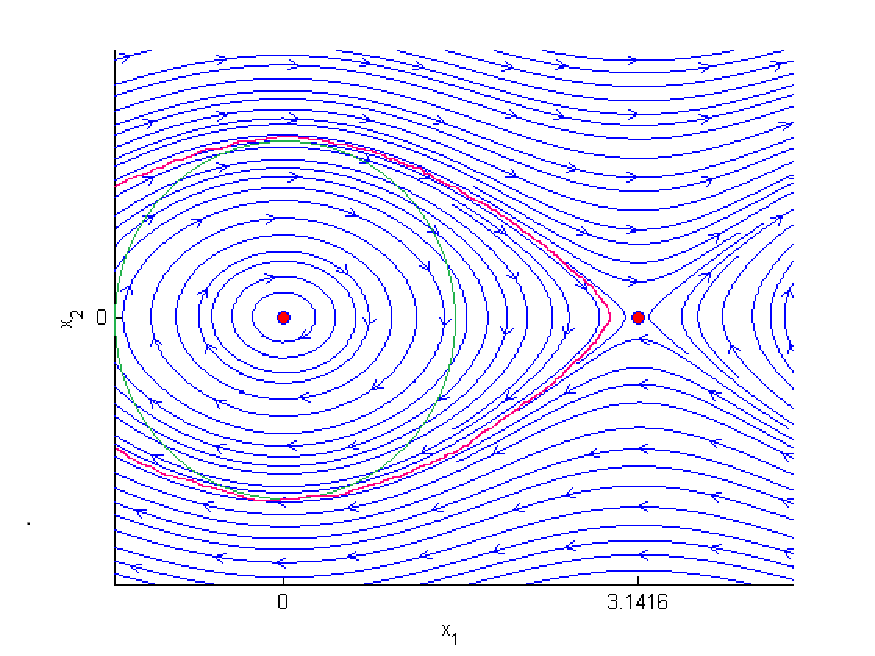
\includegraphics[width=10cm]{reg_atrac_pend}
	\caption{Estimativa da região de atração para o exemplo do pêndulo simples sem atrito}
	\label{fig:reg_atrac_pend}
\end{figure}
O domínio de atração completo deste ponto do equilíbrio situado na origem está representado pela região contida pela curva de cor rosa. A curva verde, porém, representa a estimativa do domínio de atração a qual será objeto de estudo deste capítulo.

Observe que, como o atrito é desconsiderado, a energia total do sistema permanece constante, como já visto anteriormente, a qual pode ser representada por $E(x) = c$, e forma um contorno fechado em torno da origem do plano de estados. Quando se considera o atrito, $E(x)$ se comporta como uma espiral, que se aproxima cada vez mais da origem. Para cada instante de tempo $E(x)$ vai diminuindo mais, até que alcança a origem do plano de estados. A estimativa do domínio de atração, neste caso, consiste em obter o raio $c$ máximo para o qual o sistema permanece estável para qualquer instante de tempo. De forma semelhante, Lyapunov provou que a função quadrática $V(x)$ contínua no tempo, existe uma região no plano de estados tal que $V(x) < c$ quando $\dot{V}(x) < 0$. A superfície expressa por $V(x) = c$ é conhecida como superfície de Lyapunov, para algum $c > 0$ \cite{bookkhalil:2003}.

A superfície de Lyapunov sempre estará em torno da origem do plano de estados e pode apresentar forma elipsoidal ou circular. Com base nesta afirmação, pode-se concluir que o conjunto de todos os vetores $x$ tais que $V(x) = c$, $c$ constante positivo qualquer, formam uma elipse quando a matriz simétrica $P$ da função de Lyapunov for definida positiva ($P > 0$) \cite{bookboydl:1994}. Os semi-eixos da elipse são $1/\sqrt(\lambda_i)$, em que $\lambda_i$ são os autovalores de $P/c$.

Portanto, o domínio de atração é dado pelo maior subnível da função de Lyapunov contido na região de estados limitada pelos limitantes das variáveis de estados para a qual o sistema é estável. Logo, se existem matrizes $P(\alpha) = P(\alpha)' > 0$ e $V(x) = x'P(\alpha)x$ tal que $\dot{V}(x) < 0$, então o maior conjunto contido no politopo $\chi$, em que $\chi$ é o politopo para o qual $\dot{V}(x) < 0$, é definido por
\begin{equation} \label{eq:Omega}
\Omega = \{x \in \rm I\!R^{n} | x'P(\alpha)x \leq 1\}
\end{equation}

As subseções a seguir apresentam duas abordagens para a obtenção da melhor estimativa da região de atração de sistemas com a origem como um ponto localmente assintoticamente estável.

\subsection{Primeira abordagem para obtenção da estimativa da região de atração}

Uma outra representação para o poliedro $\chi$, que equivale ao politopo dentro do qual se obteve o modelo do sistema, é dada por
\begin{equation}\label{eq:anothe_rep_of_chi}
\chi = \{x \in \rm I\!R^{n} | Qx \preceq \textbf{q}\}
\end{equation}
em que $Q\in\rm I\!R^{g\times n}$, $n\leq g$, $rank(Q) = n$, $\textbf{q} \in \rm I\!R^{n}$, $q_{(i)} > 0$, tal que $q_{(i)}$ é cada elemento de $\textbf{q}$, com $0 \in \chi$.
\begin{observation}
	Para qualquer vetor $x \in \rm I\!R^{g}$, $x \succeq 0$ significa que todos os componentes de $x$, denotados $x_{(i)}$ são não negativos. Para $x$, $y \in \rm I\!R^{n}$, $x \succeq y$ implica que $x_{(i)} - y_{(i)} \geq 0$, para todo $i = 1,\hdots, n$. Além disso, $A_{(i)}$ refere-se à i-ésima linha da matriz $A$.
	
	Observe que pode-se também ter
	\begin{equation}\label{eq:another_rep_of_chi}
	\chi = \{x \in \rm I\!R^{n} |-\mu\preceq x \preceq\mu\}
	\end{equation}
	onde $\mu \in \rm I\!R^{n}$ e $\mu{(i)} > 0, i = 1, \hdots,n$.
	De fato, os vértices $x^k$ são obtidos de $\mu$ pela combinação linear\cite{article:tarbouriech:2009}
	\begin{equation*}
	x^k = D_j\mu,\quad j =1,\hdots,2^n
	\end{equation*}
	onde $D_j, j = 1,\hdots,2^n$ são matrizes diagonais no domínio $\rm I\!R^{n \times n}$, constituídas por todas as combinações  formadas com $1$ e $-1$.
\end{observation}
Assim, uma estimativa da região de atração para o sistema não linear \ref{eq:nonlinear_system_cap_stability} pode ser obtida por um problema de minimização, conforme enuncia o teorema proposto a seguir.
	\begin{theorem}[Estimativa para região de atração] \label{th:reg_atrac_1}
		Se existem matrizes $P(\alpha) = P(\alpha)' > 0$, $X(\alpha)$, 
		$T$, um  escalar $\gamma >0$ e dado os parâmetros de ponderação $\omega_1$ e $\omega_2$ tais que
		\begin{equation}\label{eq:another_condition_1}
		min\{\omega_1Trace(T) +\omega_2\gamma\}
		\end{equation}
		sujeito a
		\begin{equation}\label{eq:th1_stability2}
		A(\alpha)'P(\alpha) + P(\alpha)A(\alpha) + Q(\gamma)J(\theta)A(\alpha) + X(\alpha)\textbf{1}'J(\theta)A(\alpha) + A(\alpha)'J(\theta)'\textbf{1}X(\alpha)' < 0
		\end{equation}
		\begin{equation}\label{eq:another_condition_3}
		\begin{bmatrix}P(\alpha)\mu_{(i)}&I^{(i)'}\\\textbf{*}&\gamma\mu{(i)}\end{bmatrix} \geq 0,\quad i = 1, ..., n
		\end{equation} 
		\begin{equation}\label{eq:another_condition_2}
		\begin{bmatrix}T&P(\alpha)\\P(\alpha)&P(\alpha)\end{bmatrix} \geq 0,
		\end{equation}	
		para todo $\alpha \in \Lambda_r$, $\theta \in \Lambda_{\vartheta}$ e $\gamma \in\Lambda_{\nu}$, 
		então 
		a origem é um ponto de equilíbrio assintoticamente localmente estável
		para o sistema não linear \ref{eq:nonlinear_system_cap_stability}
		no conjunto invariante do domínio de atração
		$\Omega = \{x\in\rm I\!R^{n}| x'P(\alpha)x \leq \gamma^{-1}\}\subseteq \chi$.
	\end{theorem}
	\begin{proof}
		Seja a função de Lyapunov $V(x)=x'P(\alpha)x$ com $P(\alpha)>0$.
		Conforme o Teorema~\ref{th:main_result}, a condição
		\ref{eq:th1_stability2} assegura $\dot{V}(x)<0$ e 
		portanto o modelo fuzzy Takagi-Sugeno \ref{eq:fuzzy_TS_system_cap_stability} é assintoticamente
		estável.
		%
		Para um politopo $\chi$ dado em \ref{eq:another_rep_of_chi},
		a condição \ref{eq:another_condition_3} assegura que
		$\Omega$ definido em \ref{eq:Omega} está incluso no politopo $\chi$,
		ou seja, $\Omega \subseteq \chi$ \cite{bookboydl:1994}.
		%
		Note que o modelo fuzzy Takagi-Sugeno \ref{eq:fuzzy_TS_system_cap_stability} somente representa 
		\ref{eq:nonlinear_system_cap_stability} para $x\in \chi$.
		Como $\Omega \subseteq \chi$, a função $V(x)$
		é localmente decrescente em $\Omega$ e $x=x(\gamma)$. Assim,
		$\Omega$ é um conjunto invariante em relação
		as trajetórias de \ref{eq:nonlinear_system_cap_stability}
		e portanto é um domínio de estabilidade do sistema não linear.
		As condições \ref{eq:another_condition_1} e \ref{eq:another_condition_2} asseguram a minimização do traço de $P(\alpha)$, 
		pois via complemento de Schur tem-se $T\geq P(\alpha)$, e portanto
		a maximização do volume de $\Omega$ \cite{bookboydl:1994}.
	\end{proof}

Veja que este teorema só é válido para sistemas com estados definidos em uma região simétrica $C$.

\subsection{Segunda abordagem para obtenção da estimativa da região de atração}

A restrição de $\Omega\subset\chi$ é válida se \cite{bookboydl:1994}
\begin{equation}\label{eq:largest_set_eq}
b_k'P(\alpha)^{-1}b_k \leq 1,\quad k = 1, \hdots, q.
\end{equation}

Observe que a Equação \ref{eq:largest_set_eq} não aparece no formato de LMI, para contornar este problema, será utilizado o Complemento de Schur, enunciado no Lema a seguir.

\begin{lemma}[Complemento de Schur para desigualdades não restritas] (Boyd, 1994) \cite{bookboydl:1994} Suponha $Q$ e $R$ matrizes simétricas. A condição
	\begin{equation}\label{eq:schur_compl_nonrestrict_1}
	\begin{bmatrix}
	Q&S\\S'&R
	\end{bmatrix} \geq 0
	\end{equation}
	é equivalente a
	\begin{equation}\label{eq:schur_compl_nonrestrict_2}
	R \geq 0,\quad Q-SR^{-1}S' \geq 0,\quad S(I-RR^{-1}) = 0.
	\end{equation}
	\label{lem:finsler_short_version_nonrestrict_inequalities}
\end{lemma}

Assim, aplicando o Complemento de Schur para desigualdades não restritas, a inequação \ref{eq:largest_set_eq} passa a equivaler à LMI

\begin{equation}\label{eq:largest_set}
\begin{bmatrix}\textbf{1}&b_k'\\b_k&P(\alpha)\end{bmatrix} \geq 0,\quad k = 1, ..., q
\end{equation}

Além disso, a região contida pelo conjunto $\Omega$ pode ser obtida maximizando o raio de $\beta > 0$ da bola centrada na origem do plano de estados contida em $\Omega$, ou seja, obtendo-se $\beta_{min}$ tal que a LMI apresentada na Equação \ref{eq:enlargment_of_largest_set} seja satisfeita.
\begin{equation}\label{eq:enlargment_of_largest_set}
P(\alpha) -  \beta I < 0
\end{equation}
Observe que as LMIs $P>0$ e $\dot{V}(x) < 0$ são suficientes para garantir a estabilidade assintótica do ponto de equilíbrio na origem. A adição das LMIs \ref{eq:largest_set} e \ref{eq:enlargment_of_largest_set} apenas garantem a obtenção de $P$ ótimo para a se obter a maior região de estimativa do domínio de atração, já se assumindo que o sistema é estável. Tem-se então o seguinte teorema proposto.
	\begin{theorem}[Outra estimativa para a região de atração]\label{th:reg_atrac_2} 
		Se existem matrizes $P(\alpha) = P(\alpha)' > 0$, $X(\alpha)$, um  escalar $\beta >0$ tais que
		\begin{equation}\label{eq:condition_1}
		min \quad \beta
		\end{equation}
		sujeito a
		\begin{equation}\label{eq:largest_set2}
		\begin{bmatrix}\textbf{1}&b_k'\\b_k&P(\alpha)\end{bmatrix} \geq 0,\quad k = 1, ..., q
		\end{equation}
		\begin{equation}\label{eq:enlargment_of_largest_set2}
		P(\alpha) -  \beta I < 0
		\end{equation} 
		e a LMI \eqref{eq:th1_stability2} sejam satisfeitas
		para todo $\alpha \in \Lambda_r$, $\theta \in \Lambda_{\vartheta}$ e $\gamma \in\Lambda_{\nu}$, 
		então $\Omega = \{x\in\rm I\!R^{n}| x'P(\alpha)x \leq 1\}\subseteq \chi$ é um conjunto invariante do domínio de atração para o sistema não linear \ref{eq:nonlinear_system_cap_stability} e a origem é um ponto de equilíbrio assintoticamente localmente estável.
	\end{theorem}
	\begin{proof}
		A prova segue linhas semelhantes da prova do Teorema~\ref{th:reg_atrac_1}. 
		A condição \ref{eq:largest_set2} implica $\Omega \subset \chi$ \cite{bookboydl:1994}. A condição \ref{eq:enlargment_of_largest_set2}
		implica $ x'P(\alpha)x < \beta ||x||$ e portanto a curva de nível
		$x'P(\alpha)x=1$ contém a esfera $||x||=1/\beta$ que é maximizada
		por \ref{eq:condition_1}. Dessa forma, o volume de $\Omega$ é maximizado.
	\end{proof}

\section{Exemplos numéricos}

Nesta seção serão utilizados exemplos numéricos já apresentados em capítulos anteriores, para os quais se obterá uma estimativa da região de atração.

%\subsection{Exemplo sistema de segunda ordem}\label{sec:ex2_JPJ12_cap_reg_atrac}

O Exemplo \ref{example_LPJ12} será utilizado nesta seção para se obter a estimativa do domínio de atração para o sistema linearizado em torno da origem, além da estimativa da região de atração para o três métodos de análise de estabilidade do modelo fuzzy T-S equivalente ao modelo não linear vistos no capítulo anterior. Para a estimativa do domínio de atração será aplicado, além das LMIs necessárias e suficientes para determinação da estabilidade em cada Método, o Teorema \ref{th:reg_atrac_1} ou o Teorema \ref{th:reg_atrac_2}. Estes diferentes métodos serão aplicados neste exemplo e, em seguida, seus resultados serão comparados para se reforçar a inspeção de qual dentre estes métodos seria o menos conservador. O critério para comparação utilizado será baseado na estimativa do domínio de atração para cada um dos métodos. Aquele que resultar na melhor estimativa, correspondendo à maior região para o domínio de atração, será considerado o melhor método.

\subsection{Método 1: Estabilidade do sistema com dinâmica linearizada}

Além dos métodos introduzidos no capítulo anterior, será utilizado um novo método neste capítulo, o qual consiste em obter, a partir do modelo não linear, um modelo linearizado segundo as técnicas clássicas encontradas na literatura. Nesta seção será utilizado o método de linearização por série de Taylor.

\subsubsection*{Análise de Estabilidade}

Para a análise da estabilidade do sistema linearizado será aplicada a função de Lyapunov para obtenção de uma matriz $P$ definida positiva, tal que o sistema seja estável.

Conforme estabelecido pela definição da estabilidade de Lyapunov, as LMIs necessárias para a determinação da estabilidade do sistema tal que a matriz $P$ não dependa das funções de pertinência, ou seja, para $P$ constante, equivalem a \cite{bookboydl:1994}

\begin{equation}\label{eq:LMIs_est_met_1}
\begin{cases}
P \geq 0\\
A'P + PA \leq 0
\end{cases}
\end{equation}

em que $A$ é uma matriz pertencente ao $\rm I\!R^{n \times n}$ cujos elementos independem dos estados $n$ do sistema. O  Exemplo \ref{ex:example2_LPJ12_non_linear_system}, quando na forma matricial, como visto anteriormente, possui um elemento não linear dependente do estado $x_1$. Portanto, será necessário linearizar o sistema tal que se obtenha a matriz $A$ no formato requerido por este método.

Para se obter o  modelo linearizado o Exemplo \ref{ex:example2_LPJ12_non_linear_system}, utilizou-se o método de linearização por série de Taylor em torno da origem, também conhecida como série de Maclaurin\footnote{Para se obter o modelo linearizado do sistema, obteve-se a representação deste na forma matricial $\dot{\textbf{x}} = A\textbf{x}$ e aplicou-se a função $taylor(A, x^*)$ do MatLab, em que $x^* = 0$.}.

O modelo linearizado é apresentado na Equação \ref{eq:ex_LPJ12_lin}.
\begin{equation}\label{eq:ex_LPJ12_lin}
\begin{cases}\dot{x}_1 = -2x_1 + 4x_2\\
\dot{x}_2= -(1 + \dfrac{\lambda}{2})x_1 - 2x_2
\end{cases},\qquad \lambda = 20
\end{equation}

Assim, a matriz $A$ do modelo linearizado será dada por

\begin{equation}\label{eq:ex_LPJ12_lin_A}A = \begin{bmatrix}-2&4\\-(1 + \dfrac{\lambda}{2})&-2\end{bmatrix},\qquad \lambda = 20
\end{equation}

Resolvendo as LMIs necessárias para a verificação da estabilidade do modelo linearizado, apresentadas na Equação \ref{eq:LMIs_est_met_1}, verifica-se que o sistema é estável para a região poliédrica $\chi$ e $\lambda = 20$.

\subsubsection*{Estimativa de Região de Atração}

Embora na análise de estabilidade do Método 1 tenha-se visto que o sistema é estável para toda a região $C$ para a qual os estados foram definidos, veremos que esta afirmação não é válida para todo o ponto do plano de estados, uma vez que o modelo linearizado só corresponde ao sistema não linear em pontos próximos à origem. Para tanto, será feita uma varredura do neste plano dentro da região de validade $C$ do sistema, considerando-se a modelagem não linear, e se  investigará em quais pontos a LMI $A'P + PA \leq 0$ é válida para a matriz $P$ obtida da análise de estabilidade do sistema, considerando-se $A$ a matriz do modelo não linear.

O teorema de estabilidade de Lyapunov estabelece, como visto no Teorema \ref{th:lyap_stability} no capítulo anterior que para se garantir a estabilidade assintótica local do ponto de equilíbrio situado na origem, seja $V(x)$ a função de Lyapunov definida positiva e para uma matriz $P > 0$, a variação de $V(x)$ deve ser definida negativa, ou seja, $\dot{V}(x) < 0$. Dito isto, para encontrar a região no plano de estados para a qual o Método 4, de fato, produz um resultado estável, deve-se obter primeiramente a inequação $\dot{V}(x)$.

Sabe-se que o exemplo em estudo possui o modelo não linear $\dot{x} = Ax$ como apresentado a seguir.

\begin{equation}\label{eq:ex2_LPJ12_non_linear_again_again}
\begin{cases}\dot{x}_1 = -2x_1 + 4x_2
\\-(1 + \dfrac{\lambda(1 - \sin(x_1))}{2})x_1 - 2x_2\end{cases},\qquad \lambda = 20
\end{equation}
Vimos anteriormente que, para $P$ constante, tem-se
\begin{equation*}
\dot{V} = x'A'Px +x'PAx < 0
\end{equation*}
O que equivale a
\begin{equation}\label{eq:V_dot_2xPAx}
\dot{V} = -2xPAx < 0
\end{equation}
Foi utilizada a equação \ref{eq:V_dot_2xPAx} substituído $A$ pelo correspondente do modelo não linear do sistema para se obter a região para a qual $\dot{V}(x)$ é definida negativa definida como $D = \{x | \dot{V}(x) < 0\}$. Desta forma, se obteve a região identificada na Figura \ref{fig:reg_estab_Met4}.

\begin{figure}[htbp]
	\centering
	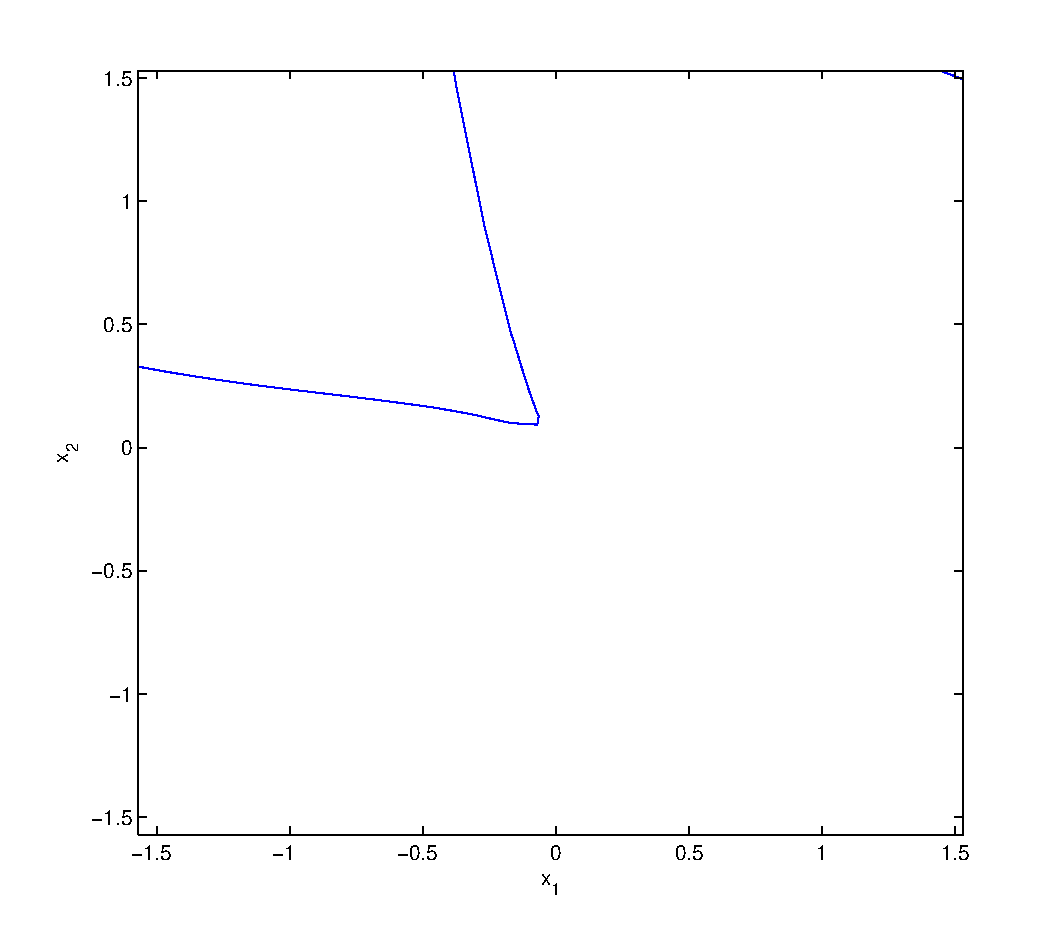
\includegraphics[width=10cm]{reg_estab_Met4}
	\caption{Região $D$ para a qual é válida a relação $\dot{V}(x) < 0$. A região está contida abaixo da curva em azul}
	\label{fig:reg_estab_Met4}
\end{figure}

Para visualizar que a região abaixo da curva azul na Figura \ref{fig:reg_estab_Met4} realmente equivale à região em que $\dot{V}(x) < 0$ para o modelo não linear, foram plotadas várias curvas para $\dot{V}(x) < y$, em que $y$ é o limitante da região representada por cada curva, Figura \ref{fig:V_dot_levels}.

\begin{figure}[htbp]
	\centering
	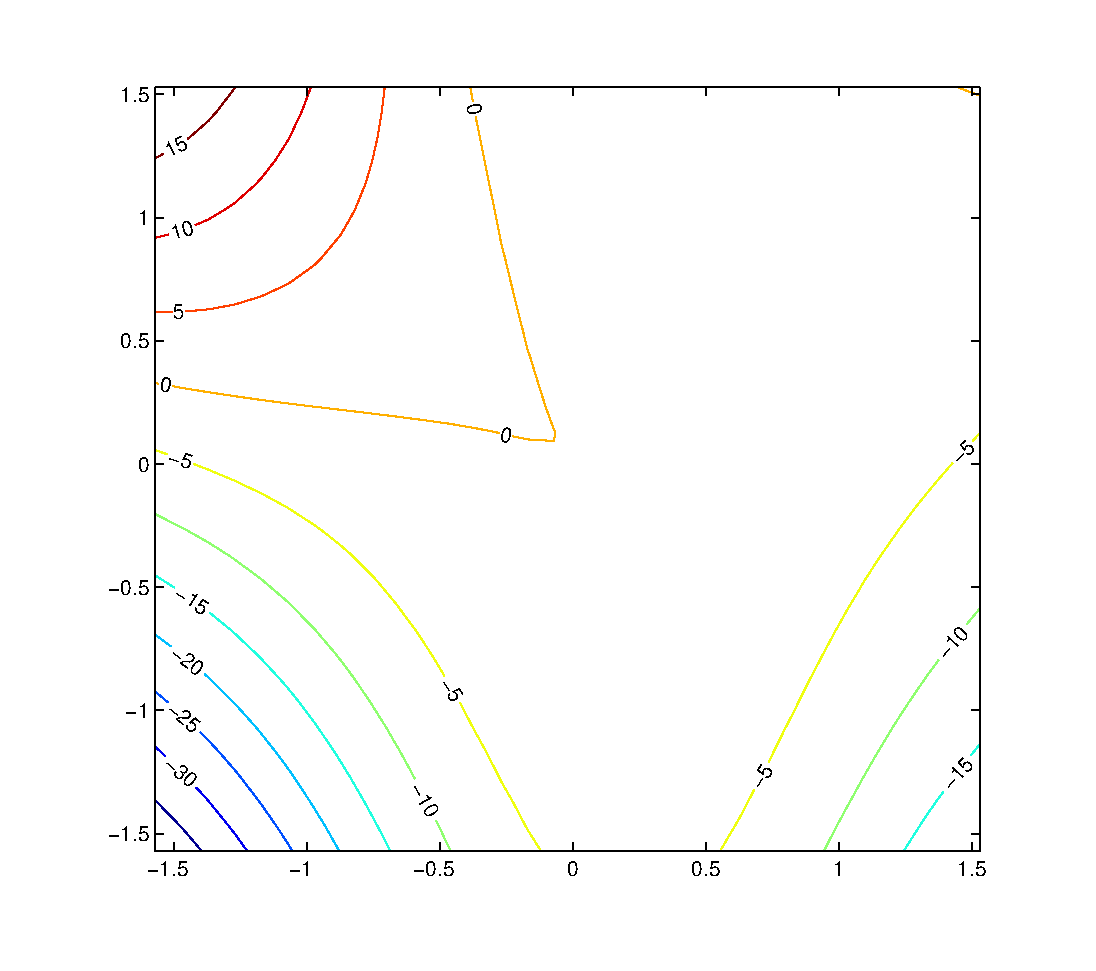
\includegraphics[width=10cm]{contour_V_dot}
	\caption{Região $D$ para diversos valores de $y$, tal que $\dot{V}(x) < y$}
	\label{fig:V_dot_levels}
\end{figure}

Como se vê na Figura \ref{fig:V_dot_levels}, a região para a qual $\dot{V}(x) < 0$, de fato, equivale à região abaixo da curva azul na Figura \ref{fig:reg_estab_Met4}.

Definida a região para a qual a análise de estabilidade é válida, estamos aptos a obter o domínio de atração para o caso apresentado no Método 1, que utiliza o modelo linearizado em torno da origem. Além das LMIs utilizadas para a análise de estabilidade vistas na Equação \ref{eq:LMIs_est_met_1}, é aplicado as condições \ref{eq:condition_1}--\ref{eq:enlargment_of_largest_set2} do Teorema \ref{th:reg_atrac_2}, de forma a se obter a melhor estimativa da região de atração. A matriz $P$ foi obtida, tal que
\begin{equation*}
P = \begin{bmatrix}0.6152&0.0000\\0.0000&0.4053\end{bmatrix}
\end{equation*}   

Como neste caso $P$ é constante, a região de atração será representada por uma região circular. Esta região é limitada no espaço $D$, no qual $\dot{V} < 0$, conforme pode ser observado na Figura \ref{fig:reg_atrac_met4}.

\begin{figure}[htbp]
	\centering
	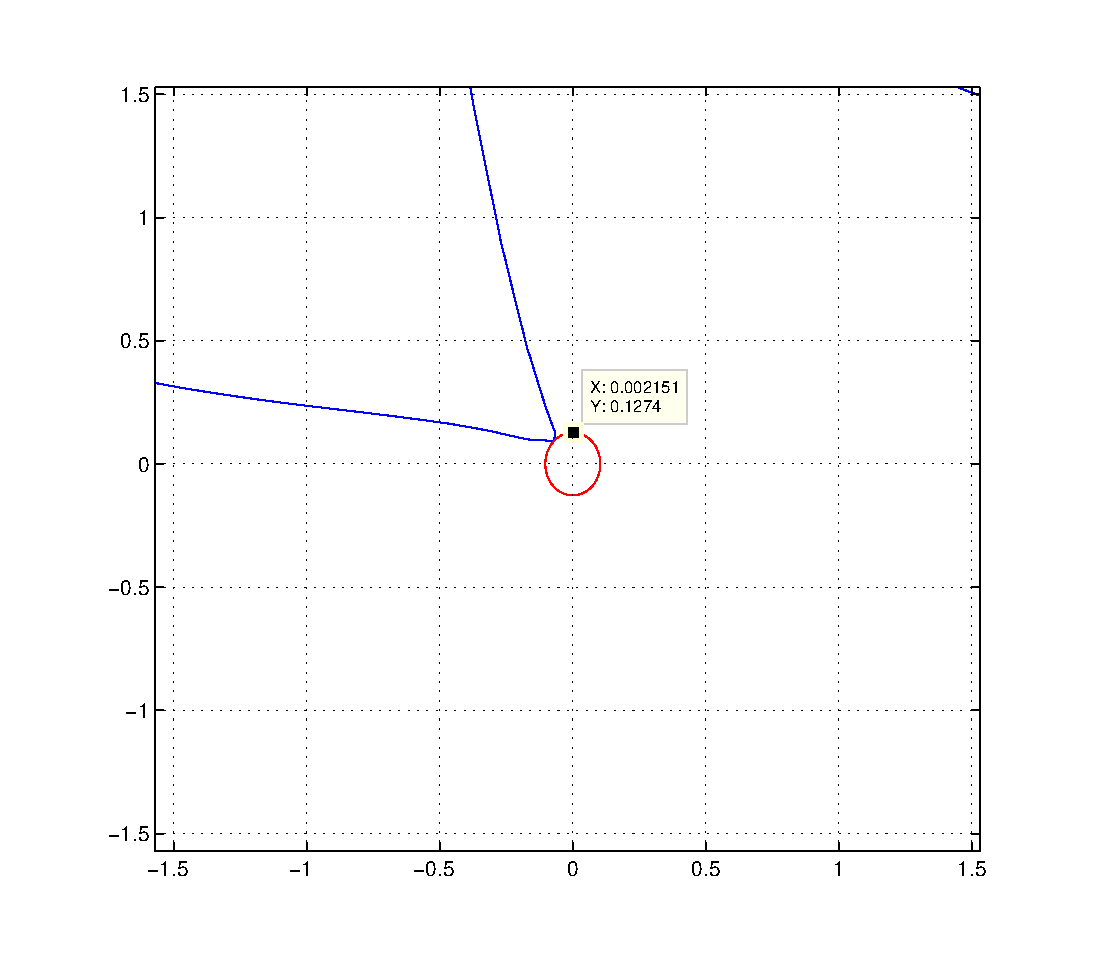
\includegraphics[width=10cm]{reg_atrac_method4}
	\caption{Estimativa da região de atração para dinâmica linearizada e $P$ constante}
	\label{fig:reg_atrac_met4}
\end{figure}

\subsection{Método 2: : (Boyd, 1994 \cite{bookboydl:1994}) Função de Lyapunov com $P$ constante e Teorema \ref{th:est_boyd}}

No capítulo anterior vimos que o modelo fuzzy Takagi-Sugeno do Exemplo \ref{example_LPJ12} somente é estável segundo o Teorema \ref{th:est_boyd} e com $\lambda = 20$ para o domínio $C_1 = 0.46C$, em que $C = \{x \in \rm I\!R^n | |x| \leq \pi/2\}$.

Como as LMIs para determinação da melhor estimativa do domínio de atração não interferem na condição de estabilidade, sabe-se que devem ser utilizadas as mesmas condições para se verificar a estabilidade que foram apresentadas no capítulo anterior por meio do Teorema \ref{th:est_boyd}. Assim, além das LMIs do Método 1 do capítulo anterior, com as condições já estabelecidas, as quais são $\lambda = 20$ e $C_1 = 0.46C$, resolveram-se também as LMIs \ref{eq:condition_1}--\ref{eq:enlargment_of_largest_set2} do Teorema \ref{th:reg_atrac_2}.

As simulações permitiram obter a matriz $P$, conforme segue.
\begin{equation*}
P = \begin{bmatrix}5.2598&0.0000\\0.0000&1.9153\end{bmatrix}
\end{equation*}

Para plotar a elipse que corresponde á superfície de nível da melhor estimativa da região de atração para este $P$ constante, utilizou-se a equação da elipse. Primeiramente determinou-se os parâmetros $b = P(1,2) = 0.0000$ e $c = P(2, 2) = 1.9153$. Além disso, assumiu-se $\gamma = 1$.
O comprimento do eixo maior a elipse equivale a $2*\sqrt(c/det(P))$, de forma que $max(x_1) = \sqrt(c/det(P)) = -min(x_1)$. Já o eixo menor foi obtido conforme a equação a seguir.
\begin{equation*}
x_2=-bx_1\pm \dfrac{\sqrt(c*\gamma-x1.^2*det(P))}{c}
\end{equation*}

A Figura \ref{fig:reg_atrac_Met1} mostra a região de estimativa do domínio de atração obtida para este método.

\begin{figure}[htbp]
	\centering
	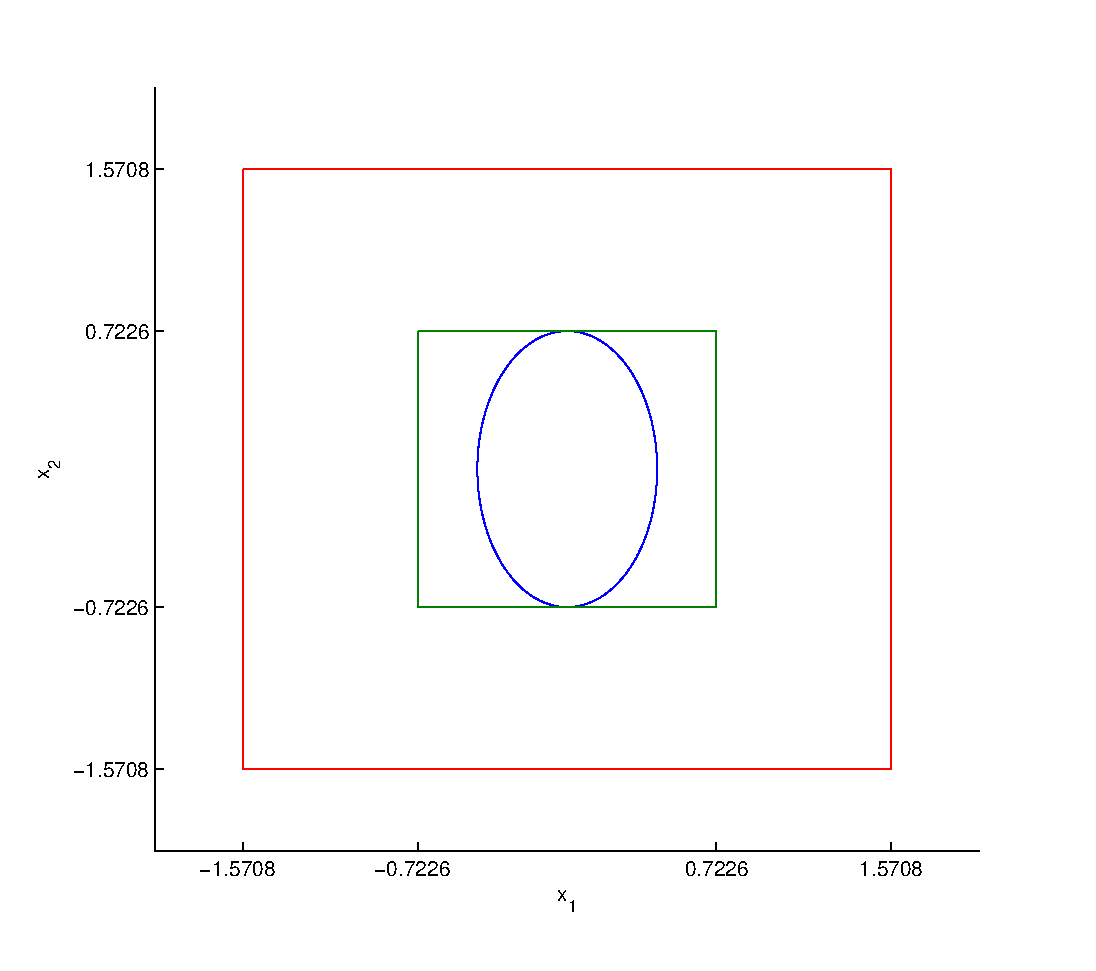
\includegraphics[width=10cm]{reg_atrac_Met1}
	\caption{Estimativa do domínio de atração do Exemplo \ref{example_LPJ12} com $\lambda = 20$ para o Método 2, curva em azul, domínio $C_1$ para a qual o sistema é localmente assintoticamente estável para este método, em verde, e domínio definido para os estados os sistema, em vermelho}.
	\label{fig:reg_atrac_Met1}
\end{figure}

\subsection{Método 3: (Mozelli, Palhares, Sousa e Mendes, 2009 \cite{MPSM:2009}) Função de  Lyapunov com $P$ dependente das funções de pertinência e limitante simples das derivadas do Teorema \ref{th:theorem_6}}

Conforme visto no capítulo anterior, este método de análise de estabilidade utiliza o artifício do limitante das derivadas simples. Os resultado obtidos previamente revelaram que a origem só é um ponto de equilíbrio estável para este método considerando-se apenas a região $C_2 = 0.51C$, em que $C = \{x \in \rm I\!R^n | |x| \leq \pi/2\}$, isto para $\lambda = 20$.

Para a obtenção da melhor estimativa da região de atração da origem para este método, consideraram-se as mesmas condições para as quais se garantiu estabilidade no capítulo anterior para $\lambda = 20$, isto é, considerou-se apenas o domínio contido em $C_2$. Assim, o sistema foi simulado para as LMIs que garantem a estabilidade para este método junto com as condições \ref{eq:condition_1}--\ref{eq:enlargment_of_largest_set2} do Teorema \ref{th:reg_atrac_2}, de forma que foram obtidas as matrizes $P_1$ e $P_2$ correspondentes aos vértices de $P(\alpha)$ conforme segue.

\begin{equation*}
P_1 =\begin{bmatrix}1.8537&0.7690\\0.7690&2.0013\end{bmatrix}\qquad P_2 = \begin{bmatrix}6.5500&-0.1329\\-0.1329&1.5609\end{bmatrix}
\end{equation*}

Por se tratarem de dois vértices, o domínio de atração agora não pode mais ser obtido conforme fora feito para os Métodos 1 e 2, que apresentavam $P$ constante, isto é, um único vértice de $P$. Assim, a curva de Lyapunov da estimativa do domínio de atração para este método foi obtida de forma tal que equivalesse à maior região contida pela interseção das superfícies de Lyapunov de cada vértice $P_i$. A Figura \ref{fig:reg_atrac_Met2} mostra esta região obtida.

\begin{figure}[htbp]
	\centering
	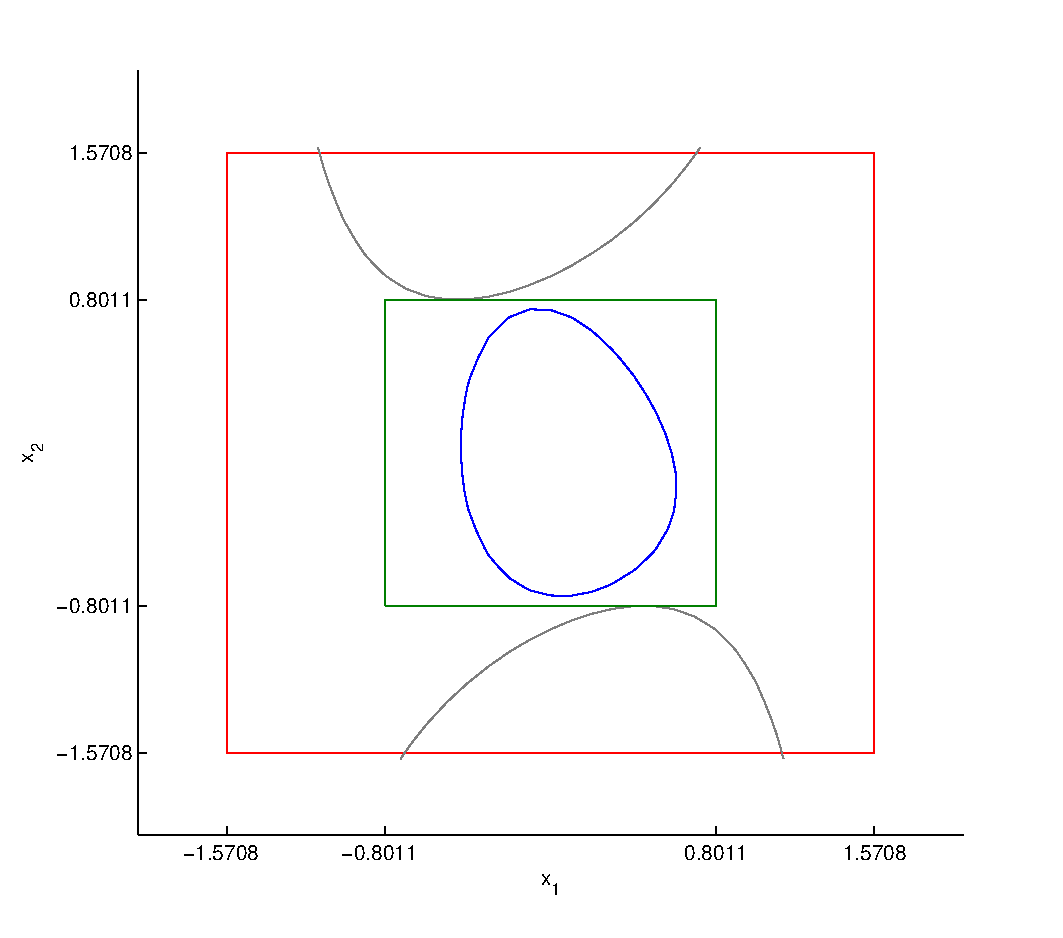
\includegraphics[width=10cm]{reg_atrac_Met2}
	\caption{Estimativa do domínio de atração do Exemplo \ref{example_LPJ12} com $\lambda = 20$ para o Método 3, curva em azul, domínio $C_2$ para a qual o sistema é localmente assintoticamente estável para este método, em verde, limitantes simples das derivadas das funções de pertinência, em cinza, e domínio definido para os estados os sistema, em vermelho}.
	\label{fig:reg_atrac_Met2}
\end{figure}

\subsection{Método 4: (Método Proposto) Função Lyapunov com $P$ dependente das funções de pertinência e Teorema \ref{th:reg_atrac_1}}

Para este Método, a melhor estimativa do domínio de atração para o Exemplo \ref{example_LPJ12} foi obtida obtendo $P$ definido positivo que satisfizesse as condições do Teorema \ref{th:reg_atrac_1}, considerando-se $\omega_1$ = $\omega_2$ = 1, de forma que se obtiveram-se os vértices $P_1$ e $P_2$ de $P(\alpha)$, conforme segue.
\begin{equation*}
P_1 = 1.0e+05 \begin{bmatrix} 0.3085&0.4474\\0.4474&2.1328\end{bmatrix}\qquad P_2 = 1.0e+05 \begin{bmatrix}1.8249& 0.1148\\ 0.1148&1.2450\end{bmatrix}
\end{equation*}

Este método tem em especial o fato de que a estimativa da região de atração é plotada para um $\gamma = 1.9666e-05$, obtido da resolução das LMIs do Teorema \ref{th:reg_atrac_1}, ao contrário do que ocorre para os demais Métodos, em que se assume $\gamma = 1$.

A Figura \ref{fig:reg_atrac_met5} apresenta a superfície da melhor estimativa do domínio de atração para o Método 5.

\begin{figure}[htbp]
	\centering
	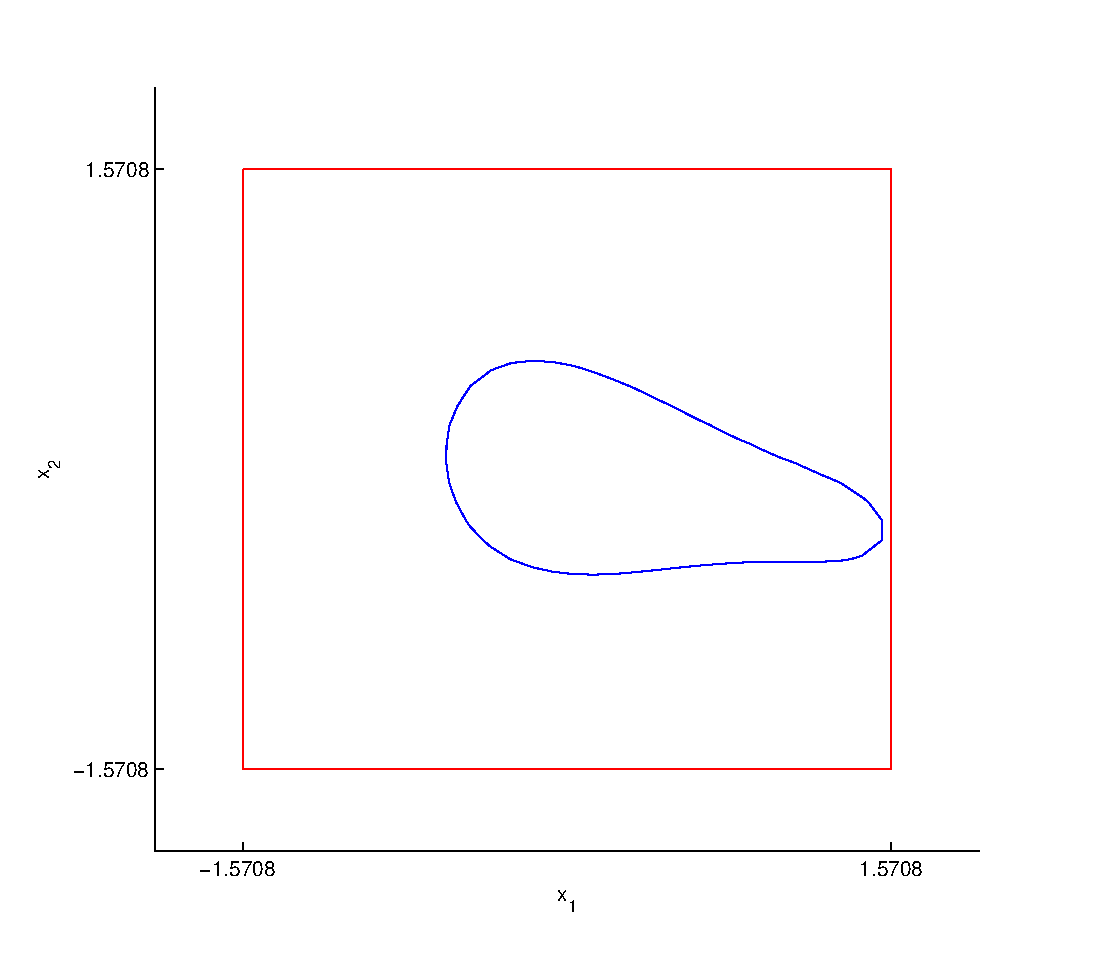
\includegraphics[width=10cm]{reg_atrac_Met5}
	\caption{Estimativa do domínio de atração do Exemplo \ref{example_LPJ12} com $\lambda = 20$ para o Teorema~\ref{th:reg_atrac_1}, curva em azul, e domínio $C$ para a qual o sistema é localmente assintoticamente estável para o Resultado Principal (Proposto), em vermelho}
	\label{fig:reg_atrac_met5}
\end{figure}

\subsection{Método 5: (Método Proposto) Função Lyapunov com $P$ dependente das funções de pertinência e Teorema \ref{th:reg_atrac_2}}

A melhor estimativa do domínio de atração para o Exemplo \ref{example_LPJ12}, assumindo-se $\lambda = 20$, para o Resultado Principal deste trabalho é obtida resolvendo-se as LMIs propostas no Teorema~\ref{th:reg_atrac_2}. Obtendo-se mais uma vez o resultado o qual indica que a origem é um ponto estável, gerando-se valores para os vértices de $P(\alpha)$ definido positivo.

Como $P(\alpha)$ é dependente das funções de associação, este possui $2$ vértices, os quais são descritos a seguir, considerando-se a condição de melhor estimativa do domínio de atração, ou seja, obtendo solução tal que satisfizesse o Teorema \ref{th:reg_atrac_2}.
\begin{equation*}
P_1 =\begin{bmatrix}0.4596&0.3295\\0.3295&1.9980\end{bmatrix}\qquad P_2 = \begin{bmatrix}1.9137&-0.1639\\-0.1639&0.4671\end{bmatrix}
\end{equation*}

A curva correspondente á melhor estimativa do domínio de atração para este método foi obtida conforme descrito no Método 2. Foi obtida a região correspondente à maior interseção entre as elipses equivalentes aos vértices de $P(\alpha)$. A Figura \ref{fig:reg_atrac_Met3} apresenta o resultado obtido para o domínio de atração obtido para este método.

\begin{figure}[htbp]
	\centering
	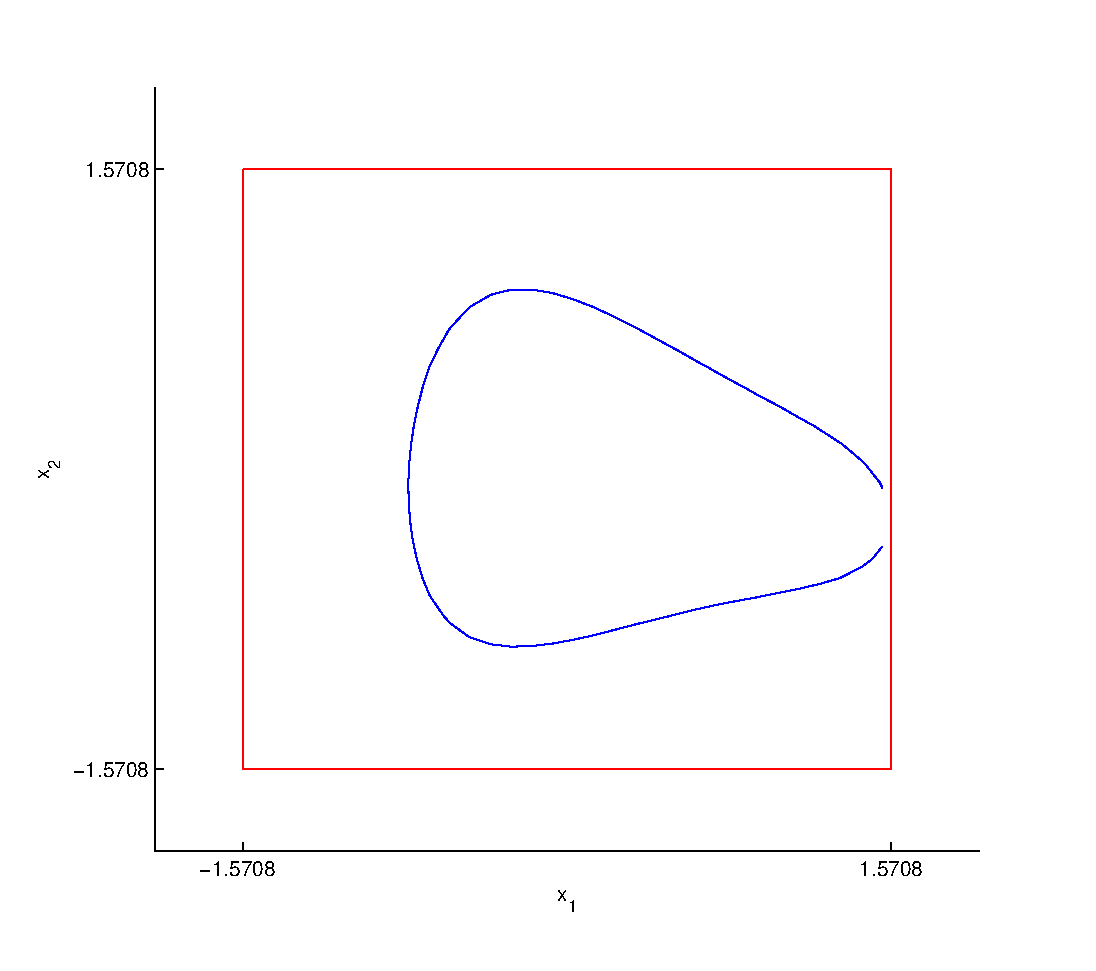
\includegraphics[width=10cm]{reg_atrac_Met3}
	\caption{Estimativa do domínio de atração do Exemplo \ref{example_LPJ12} com $\lambda = 20$ para o Resultado Principal (Proposto), curva em azul, e domínio $C$ para a qual o sistema é estável para este método, em vermelho}.
	\label{fig:reg_atrac_Met3}
\end{figure}

\subsection{Comparação entre os métodos}

Para se comparar os resultados dos cinco métodos apresentados nesta seção, como nem todas as curvas obtidas têm um formato definido como elipse ou círculo, o que dificulta os cálculos da área contida pela curva de Lyapunov obtida para cada um dos métodos, as curvas correspondentes a estas estimativas da região de atração serão plotadas em um único gráfico, de forma a se verificar visualmente qual delas cobre uma maior região no plano de estados, conforme mostra a Figura \ref{fig:reg_atrac_all_met}.


\begin{figure}[htbp]
	\centering
	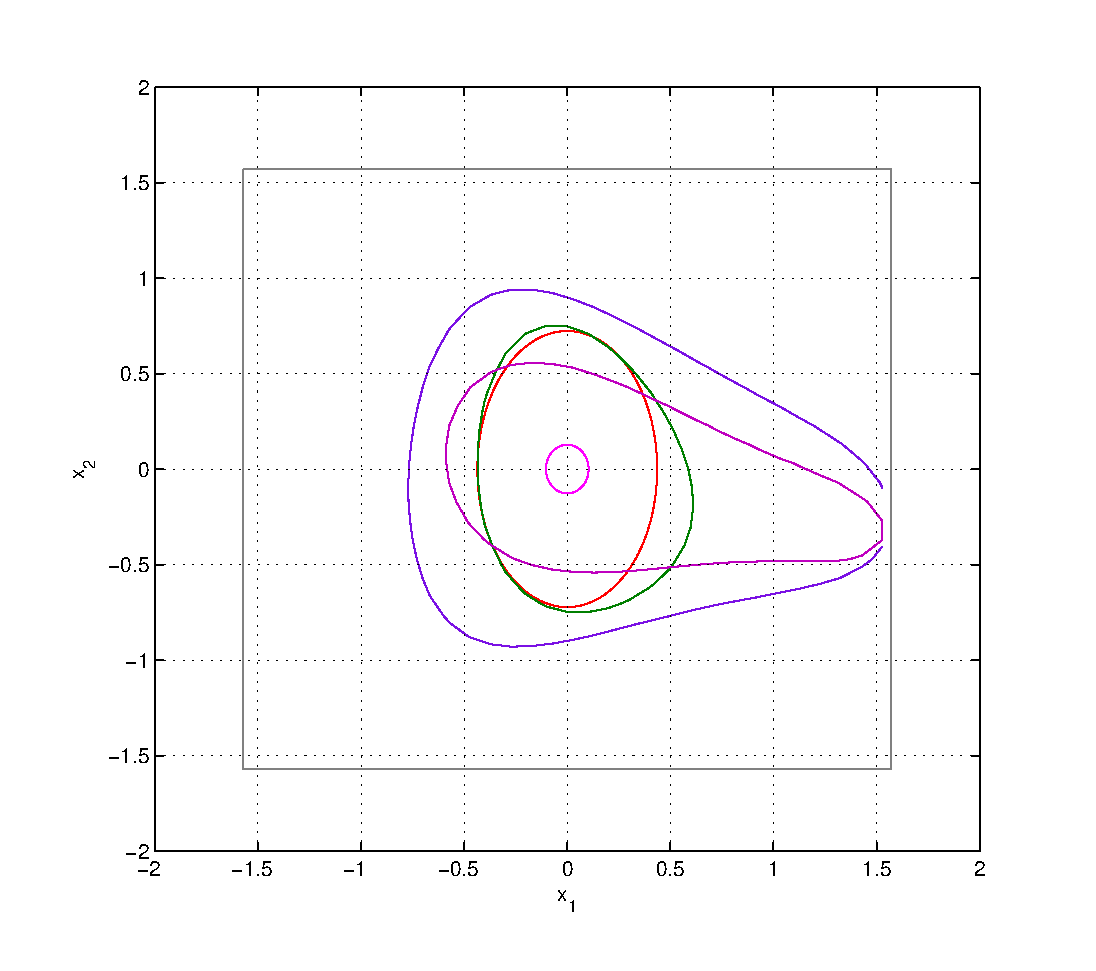
\includegraphics[width=10cm]{domain_of_attraction_all_methods}
	\caption{Estimativa do domínio de atração do Exemplo \ref{example_LPJ12} com $\lambda = 20$ para os cinco Métodos propostos nesta seção. A curva referente ao Método 1 é mostrada na cor rosa. A curva em vermelho corresponde ao  Método 2, a curva em verde equivale ao  Método 3. A curva obtida do  Método 4 aparece em roxo e curva do  Método 5, em azul. A região $C$ para a qual os estados são limitados aparece na cor cinza}
	\label{fig:reg_atrac_all_met}
\end{figure}

Na Figura \ref{fig:reg_atrac_all_met}, a região para a qual os estados estão limitados aparecem como o quadrado na cor cinza. As regiões de atração do ponto de equilíbrio na origem aparecem para os Métodos 1, 2, 3, 4 e 5 aparecem na Figura, respectivamente, nas cores rosa, vermelho, verde, roxo e azul.

O Método 1, apresentado na cor rosa, foi o que gerou o pior resultado, o que se era esperado, uma vez que a dinâmica linearizada neste método só é válida para regiões muito próximas á origem, já que o sistema foi linearizado em torno deste ponto. Todos os demais métodos foram aplicados para a dinâmica do sistema modelada segundo a estratégia de não linearidade por setor para modelos fuzzy Takagi-Sugeno.

O Método 3, que utiliza artifício dos limitantes por derivada simples se mostrou um pouco melhor que o Método 2, o qual apresenta $P$ constante. 

Ao contrário do que fora feito para os Métodos 1, 2 e 3, em que se utilizou apenas o Teorema \ref{th:reg_atrac_2} para a obtenção da melhor estimativa de região de atração, para o Resultado principal deste trabalho, obteve-se a estimativa de região de atração utilizando tanto o Teorema \ref{th:reg_atrac_1}, conforme mostra o Método 4, quanto para o Teorema \ref{th:reg_atrac_2}, segundo Método 5.
Como se pode observar na Figura \ref{fig:reg_atrac_all_met}, o método que gerou o melhor resultado para estimativa da região de atração foi o  Método 5, que equivale ao Resultado Principal proposto por este trabalho utilizando-se o Teorema  \ref{th:reg_atrac_2} e o Método 4 gerou o segundo melhor resultado. 

% \section{Exemplos}

% [UFSM]

\section{Considerações Finais}

Neste capítulo foram apresentados dois Teoremas para a obtenção da melhor estimativa de região de atração do ponto de equilíbrio situado na origem do plano de estados para sistemas dinâmicos não lineares modelados segundo o artifício de não linearidade por setor local, proposto por \cite{booktw:2003}, para obtenção de modelos fuzzy Takagi-Sugeno do sistema \cite{articlets:1985}. Tentou-se obter a maior região dentro do espaço de estados para a qual o sistema é estável e para a qual, uma vez que as respostas, iniciadas em qualquer ponto da região do plano de estado limitada pelas restrições dos estados do sistema, adentrem esta região de atração, jamais consiga sair desta.

Para verificar se, de fato, o Resultado Principal (Proposto) neste trabalho fornecia o melhor resultado para a estimativa do domínio de atração do ponto de equilíbrio na origem, utilizaram-se outros três métodos. Dois destes métodos já haviam sido explorados no capítulo anterior, em que se analisou a estabilidade de pontos de equilíbrio para sistemas com dinâmica fuzzy T-S e o outro método consistiu na análise de estabilidade e obtenção da estimativa de região de atração para o sistema linearizado em torno da origem.

O primeiro Método utilizado para comparação consistiu no modelo linearizado em torno da origem e com $P$ constante. Este método, embora tenha se apresentado como estável para toda a região definida para os estados do sistema, produz o pior resultado de estimativa de região de atração, obtida com o uso do Teorema \ref{th:reg_atrac_2}, dado que só é válido para regiões muito próximas à origem, como se verificou varrendo-se a região para a qual relação $\dot{V} < 0 $ é válida para o sistema não linear.

Para dois métodos já vistos no capítulo anterior, com exceção do Resultado Principal (Proposto), que utilizam Estabilidade de Lyapunov com P constante, proposto por (Boyd, 1994 \cite{bookboydl:1994}) e Estabilidade de Lyapunov com $ P(\alpha)$ e limitante por derivada simples, segundo proposto por (Mozelli, Palhares, Sousa e Mendes, 2009 \cite{MPSM:2009}), respectivamente, foram obtidas as estimativas de região de atração utilizando-se o Teorema \ref{th:reg_atrac_2}. Este primeiro Método se mostrou pior que o segundo, uma vez que a região estimada foi menor. Porém, ambos apresentaram resultados piores que os do Teorema \ref{th:main_result}, que consiste no resultado principal deste trabalho. Estes resultados foram piores, tanto quando comparados utilizando-se o Teorema \ref{th:reg_atrac_1}, quanto o Teorema \ref{th:reg_atrac_2} para a estimativa da região de atração. 

Para o caso dos Métodos 4 e 5, correspondentes ao resultado principal, o que gerou o melhor resultado, que se permitiu obter a maior estimativa de região de atração dentre todos os métodos vistos, foi o Método 5.